\documentclass{beamer}

\usepackage{graphicx}

\usecolortheme[named=blue]{structure}

\mode<presentation>
{
  \usetheme{Warsaw}
  \setbeamercovered{transparent}
  \setbeamertemplate{items}[ball]
  \setbeamertemplate{theorems}[numbered]
  \setbeamertemplate{footline}[frame number]
  
% custom colors
  \setbeamercolor{structure}{fg=red!90!black}
  
  \setbeamerfont{section number projected}{%
  	family=\rmfamily,series=\bfseries,size=\normalsize
  }
  \setbeamercolor{section number projected}{bg=red,fg=white}
  \setbeamercolor{frametitle in head}{fg=Brown,bg=Brown!20}
  
}

% \usecolortheme{spruce}

\usepackage{beamerthemesplit}
\usepackage{graphics}
\usepackage{graphicx}
\usepackage{hyperref}
\usepackage{color}
\usepackage{listings}
\usepackage[utf8]{inputenc}

\newcommand{\code}[1]{\texttt{\small{#1}}}
\hypersetup{%
  colorlinks=true,
  urlcolor=red,
  linkcolor=red,
  pdfborderstyle={/S/U/W 1}
}

\definecolor{javared}{rgb}{0.6,0,0} % for strings
\definecolor{javagreen}{rgb}{0.25,0.5,0.35} % comments
\definecolor{javapurple}{rgb}{0.5,0,0.35} % keywords
\definecolor{javadocblue}{rgb}{0.25,0.35,0.75} % javadoc

\lstdefinelanguage{scala}{
  morekeywords={abstract,case,catch,class,def,%
    do,else,extends,false,final,finally,%
    for,if,implicit,import,match,mixin,%
    new,null,object,override,package,%
    private,protected,requires,return,sealed,%
    super,this,throw,trait,true,try,%
    type,val,var,while,with,yield},
  otherkeywords={=>,<-,<\%,<:,>:,\#,@,>,<},
  sensitive=true,
  morecomment=[l]{//},
  morecomment=[n]{/*}{*/},
  morestring=[b]",
  morestring=[b]',
  morestring=[b]"""
}
\lstset{
%   frame=tb,
  language=Scala,
  aboveskip=3mm,
  belowskip=3mm,
  columns=flexible,
  basicstyle=\ttfamily\small,
  keywordstyle=\color{javapurple}\bfseries,
  stringstyle=\color{javared},
  commentstyle=\color{javagreen},
  morecomment=[s][\color{javadocblue}]{/**}{*/},
  numbers=none,
  numberstyle=\tiny\color{black},
  stepnumber=2,
  numbersep=10pt,
  showspaces=false,
  showstringspaces=false,
  tabsize=4
}

\newcommand{\screenshot}[1]{\centerline{%
    \includegraphics[height=7.8cm,transparent]{#1}}}  % 7.8in

\title
  [Wollok: en el aula y más allá]
  {Wollok: en el aula y más allá}
\author[Passerini, Fernandes, Tesone]{%
  Javier Fernandes\inst{1,2} \and
  Nicolás Passerini\inst{1,2,4} \\
  Pablo Tesone\inst{3,1,2,4} \and
  Débora Fortini\inst{1,4} \\
  Nahuel Palumbo\inst{4} \and
  Juan Contardo\inst{4} \and
  Carlos Raffellini\inst{4}
}  

\institute{
  \inst{1}Universidad Nacional de Quilmes \\
  \inst{2}Universidad Nacional de San Martin \\
  \inst{3}Universidad Nacional del Oeste \\
  \inst{4}Universidad Tecnológica Nacional - F.R. Buenos Aires.
}

\date[WISIT 2015]{\small Workshop de Ingeniería en Sistemas y Tecnologías de la Información \\ 19/09/2015}
\subject{Computational Sciences}

%\logo{\includegraphics[height=1.0cm]{fsu_logo.pdf}}

\begin{document}
  \frame
  {
    \titlepage
  }

  \frame
  {
    \frametitle{Agenda}
    \tableofcontents
  }

\section{Introduccion}
\defverbatim[colored]\helloWorldJava{
\begin{lstlisting}[language=Java]
		package examples;
		
		public class HelloWorld {
			public static void main(String[] args) {
				System.out.println("Hello World");
			}
		}
\end{lstlisting}
}

\frame{
	\frametitle{Introducción}
	\framesubtitle{¿Por qué es difícil aprender OOP?}	
	\begin{itemize}
    \item Enfoque en un lenguaje particular
    \item Demasiados conceptos
    \medskip
    \helloWorldJava
    \pause
    \item \textbf{Entornos de desarrollo} limitados o inadecuados
    \item Aprender a programar exige \textbf{aprender a abstraer}
	\end{itemize}
}

\frame{
	\frametitle{Introducción}
	\framesubtitle{Antecedentes}
	
\includegraphics[width=9,
			 	height=9,natwidth=66,natheight=50]{images/ozono-icon.png}
	\textbf{Ozono} \hfill \texttt{\footnotesize
	\href{http://ozono.uqbar-project.org/}{http://ozono.uqbar-project.org/}}
	\begin{itemize}
		\item Basado en Smalltalk
		\item \textbf{Recorrido incremental}
		\\\hspace{2em} Metamodelo simplificado: sin clases ni herencia
		\\\hspace{2em} Foco en objeto - mensaje - referencia - polimorfismo
		\item Herramientas de visualización de código
		\\\hspace{2em} Diagramas de objetos / clases
	\end{itemize}
	
	\pause\bigskip
	
\includegraphics[width=9,
			 	height=9,natwidth=313,natheight=365]{images/gobstones-icon.png}
	\textbf{Gobstones} \hfill \texttt{\footnotesize
	\href{http://www.gobstones.org/}{http://www.gobstones.org/}}
	\begin{itemize}
		\item Cuidadosa selección de los elementos sintácticos
		\item Elimina la necesidad de entrada-salida
		\item Separación entre elementos con efecto y elementos puros
	\end{itemize}
}

\frame{
	\frametitle{Introducción}
	\framesubtitle{¿Qué es Wollok?}
	\begin{itemize}
	 \item Lenguaje + muchas herramientas
	 \item Optimizados para la enseñanza
	 \item Cercanos a las herramientas profesionales \emph{mainstream}
	 \item Proyecto abierto
	\end{itemize}
	
	\begin{center}
		\begin{figure}
			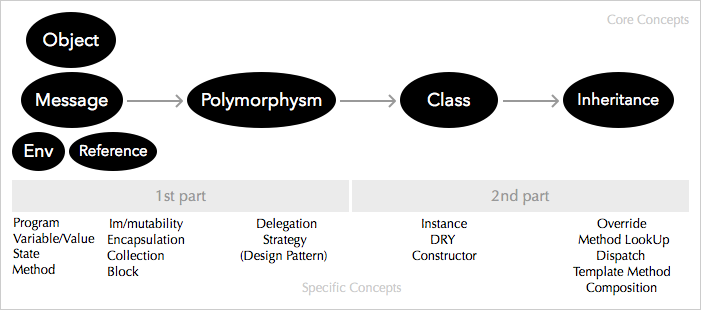
\includegraphics[width=1\textwidth,height=0.6\textheight,natwidth=701,natheight=310]{images/wollok-learning-path.png}
		\end{figure}
	\end{center}
	
}

\frame{
	\frametitle{Introducción}
	\framesubtitle{¿Qué es Wollok? - Pensado para enseñar}
	\begin{itemize}
		\item Sintaxis cuidada 
			\begin{itemize}
			  \item selección de keywords
			  \item return obligatorio
			  \item énfasis en objetos y mensajes
			  \hspace{2em} {\small (aunque no todo es objeto mensaje)}
			\end{itemize}
		\item Combina object-based con class-based programming
		\item APIs minimalistas (ej: colecciones)
		\item Import system
	\end{itemize}
}

\frame{
	\frametitle{Introducción}
	\framesubtitle{¿Qué es Wollok? - Cercano al mainstream}
	\begin{itemize}
		\item Ambiente de objetos basado en archivos
		\item Framework de testing integrado
		\item Literales para listas y conjuntos (próximamente diccionarios)
		\item Manejo de excepciones 
	\end{itemize}
}

\section{Desarrollo de Wollok}
\frame{
	\frametitle{Desarrollo de Wollok}	
	\begin{itemize}
		\item OpenSource: LGPLv3 
		\item Stack: 
\includegraphics[width=9,
			 	height=9,natwidth=32,natheight=32]{images/eclipse-icon.png} Eclipse XText +
			 	Xtend Lang
		\item SCM:
			\begin{itemize}
			  	\item \textbf{Código}: 
\includegraphics[width=9,
			 	height=9,natwidth=16,natheight=16]{images/github-icon.png} GitHub
			  	(\href{https://github.com/uqbar-project/wollok}{uqbar-project/wollok})
			 	\item \textbf{Build}: Maven + Tycho
			 	\item \textbf{Continuous Integration}:
			 	
\includegraphics[width=9,
			 	height=9,natwidth=50,natheight=50]{images/travis-ci-icon.png} Travis
			 	\item \textbf{Continuous Deployment}
			 	\item \textbf{Coverage}: coveralls + jacoco
			 \end{itemize}
		\item Testing \& TDD
	\end{itemize}
}

\frame{
	\frametitle{Desarrollo de Wollok}
	\framesubtitle{Continuous Integration \& Deployment}	
	\begin{itemize}
	  	\item \textbf{GitFlow}
	  		\begin{itemize}
	  		  \item Feature Branches
	  		  \item Pull-Requests
	  		  \item $dev \rightarrow master \leftarrow  hotfixes$ 
			\end{itemize}	 
		\item \textbf{Integration}:
			\begin{itemize}
			  \item Travis
			  \item compile, test, coverage, deploy
			\end{itemize}
		\item Deployment:
				\begin{itemize}
				  \item \textbf{Productos} (IDE): multiples pataformas
				  \item \textbf{Update Sites}
				  \item \textbf{WDK}
				  \item 2 Ambientes: Stable \& Dev
				\end{itemize}
	\end{itemize}
}

\frame{
	\frametitle{Desarrollo de Wollok}
	\framesubtitle{Testing \& TDD}	
	\begin{itemize}
	  	\item 87\% Cobertura 	
	  	\item \textbf{Runtime}      % SCREEN: ACA MOSTRAMOS UN SCREENSHOT DE UN TEST
	  		\begin{itemize}
	  		  \item Testean ejecución
	  		  \item Interprete
	  		  \item \textbf{JUnit + iDSL}
			\end{itemize}	 
		\item \textbf{Estáticos}
			\begin{itemize}
			  \item \textbf{Chequeos}: XPect  % SCREEN: ACA MOSTRAMOS UN TEXT XPECT
			  \item \textbf{Type System}: JUnit + iDSL
			  \item \textbf{Autocomplete}: XPect
			  \item \textbf{Formateo}: JUnit + iDSL
			\end{itemize}
		\item \textbf{Pendientes}
			\begin{itemize}
			  \item Quick-Fixes
			  \item Refactors
			\end{itemize}
	\end{itemize}
}

\frame{
	\frametitle{Testing \& TDD}
	\framesubtitle{Runtime}
	Testeo del Intérprete
	\begin{center}
		\begin{figure}
			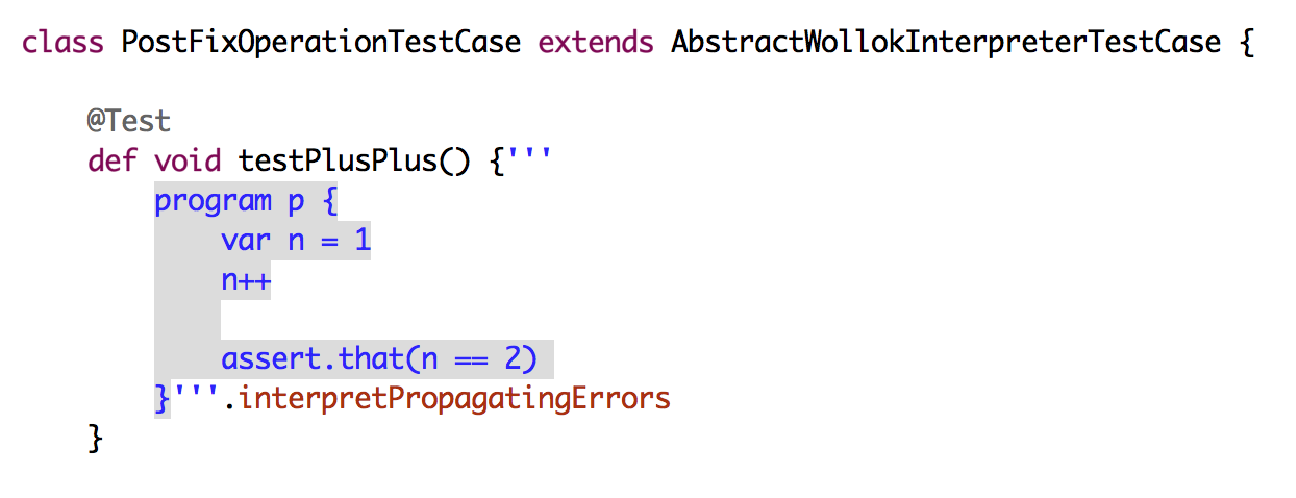
\includegraphics[width=1\textwidth,height=0.6\textheight,natwidth=836,natheight=444]{images/wollok-tests-runtime.eps}
		\end{figure}
	\end{center}
}

\frame{
	\frametitle{Testing \& TDD}
	\framesubtitle{Chequeos Estáticos}
	Testeo de Chequeos Estáticos
	\begin{center}
		\begin{figure}
			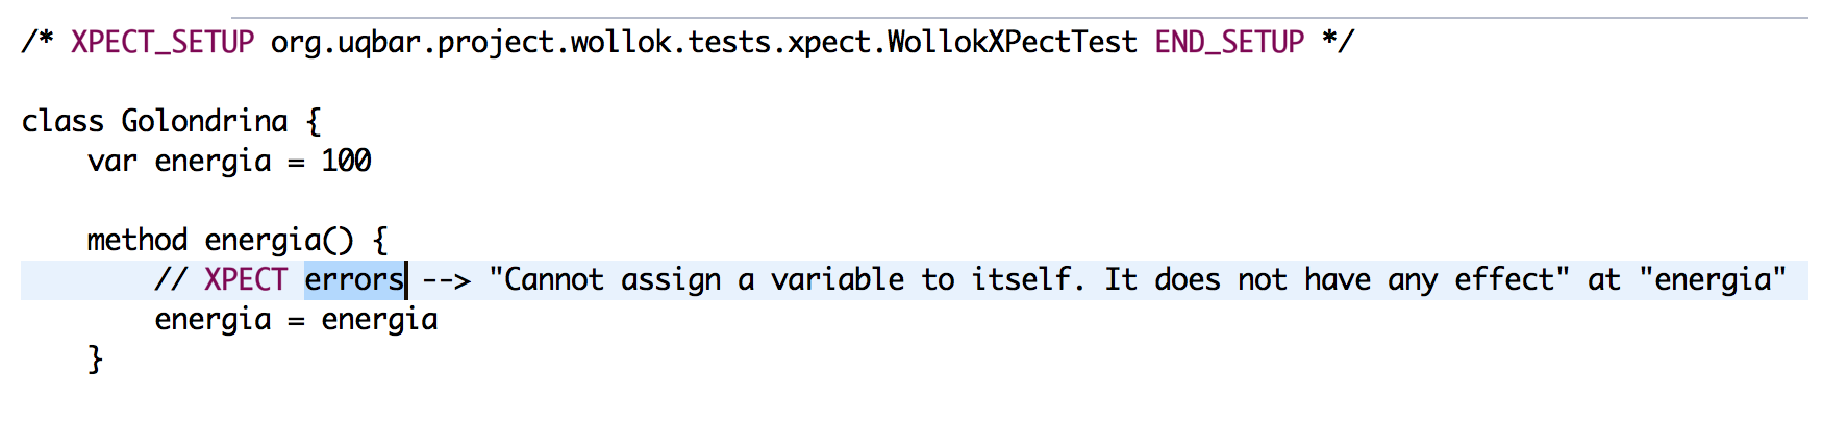
\includegraphics[width=1\textwidth,height=0.45\textheight,natwidth=1720,natheight=372]{images/wollok-tests-checkeos.eps}
		\end{figure}
	\end{center}
}

% \frame{
% 	\frametitle{Testing \& TDD}
% 	\framesubtitle{Type System}
% 	Testeo del Type System
% 	\begin{center}
% 		\begin{figure}
% 			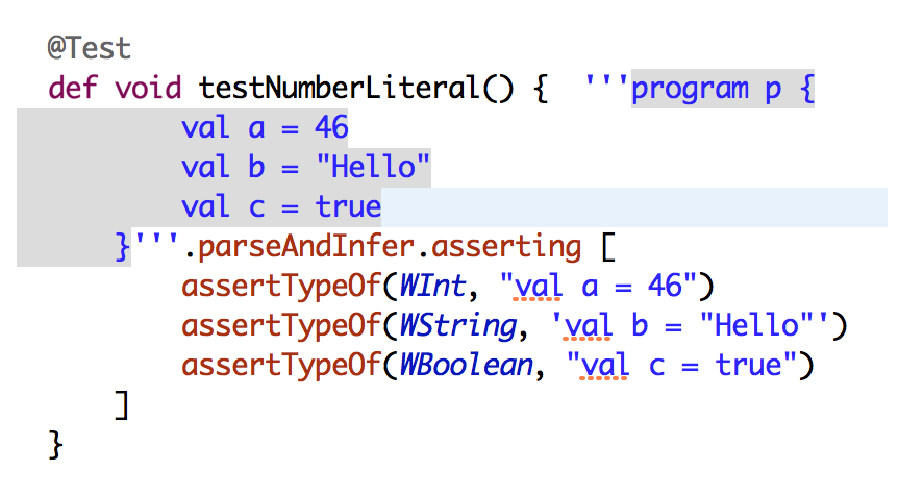
\includegraphics[width=1\textwidth,height=0.6\textheight,natwidth=836,natheight=444]{images/wollok-tests-typesystem.eps}
% 		\end{figure}
% 	\end{center}
% }

%
% FEATURE AVANZADOS
%

\section{Features Avanzados}
\frame{
	\frametitle{Features Avanzados}	
	\begin{itemize}
    \item Debugger
    \item Diagramas: Clases y Objetos
    \item Tests
    \item ContentAssist y QuickFixes
    \item Sublime Plugins 
    \item I18N
	\end{itemize}
}

\frame{
	\frametitle{Features Avanzados}
	\framesubtitle{Debugger}
	Debugger
	\begin{itemize}
	    \item UI integrada a Eclipse Debug
	    \item Breakpoints: agregar, remover, deshabilitar, etc
	    \item Step, into, out 
	    \item Inspeccionar variables
	    \item Diagrama de Objetos
	\end{itemize}
}

\frame{
	\frametitle{Features Avanzados}
	\framesubtitle{Tests}
	Tests
	\begin{center}
		\begin{figure}
			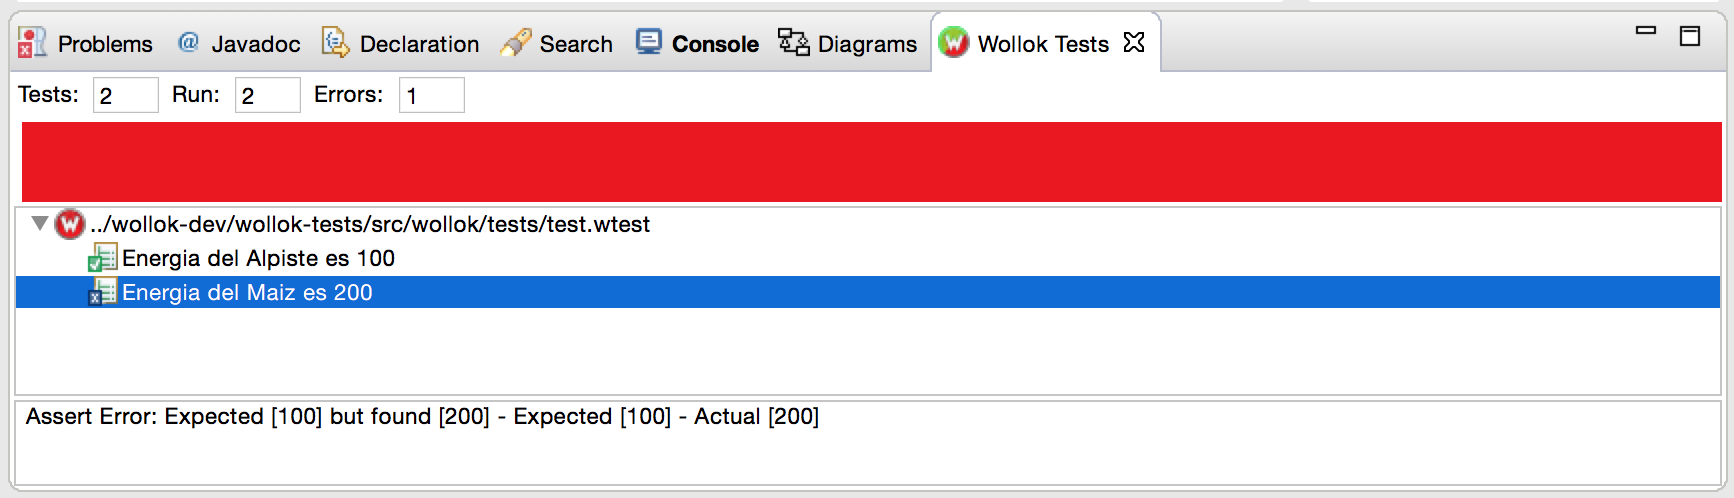
\includegraphics[width=1\textwidth,height=0.6\textheight,natwidth=1734,natheight=498]{images/tests.png}
		\end{figure}
	\end{center}
}

\frame{
	\frametitle{Features Avanzados}
	\framesubtitle{Soporte para Sublime}
	Soporte para Sublime
	\begin{itemize}
	    \item WDK
	    	\begin{itemize}
	    		\item No IDE
	    		\item $\sim70$MB (vs $\sim140$)
	    		\item Headless: wchecker, winterpreter, wtest
	    	\end{itemize}
	    \item Syntax highlight
	    \item Templates 
	    \item Linter
	\end{itemize}
}


\frame{
	\frametitle{Sublime Support}
	\framesubtitle{Syntax Highlight}	
	\begin{center}
		\begin{figure}
			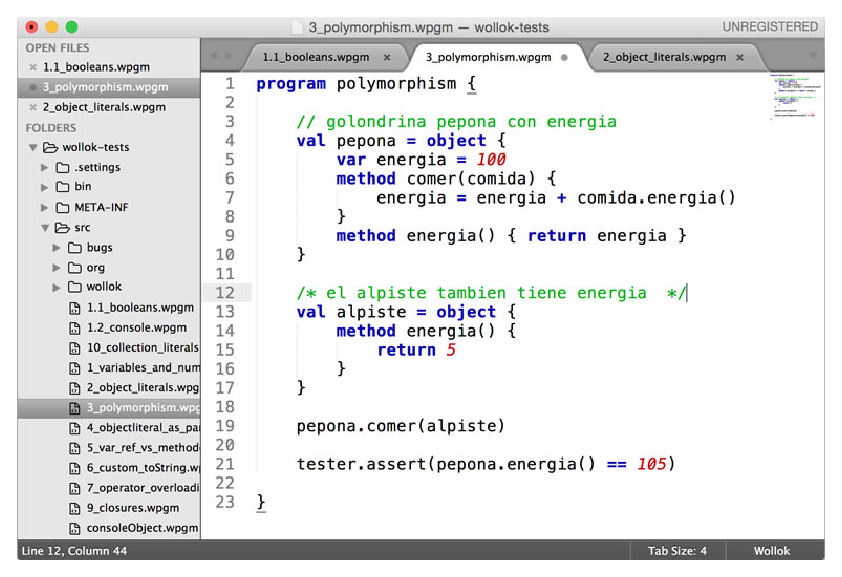
\includegraphics[height=0.8\textheight,natwidth=800,natheight=561]{images/wollok-wisit-sublime-syntax.eps}
		\end{figure}
	\end{center}
}

\frame{
	\frametitle{Sublime Support}
	\framesubtitle{Linter}
	\begin{center}
		\begin{figure}
			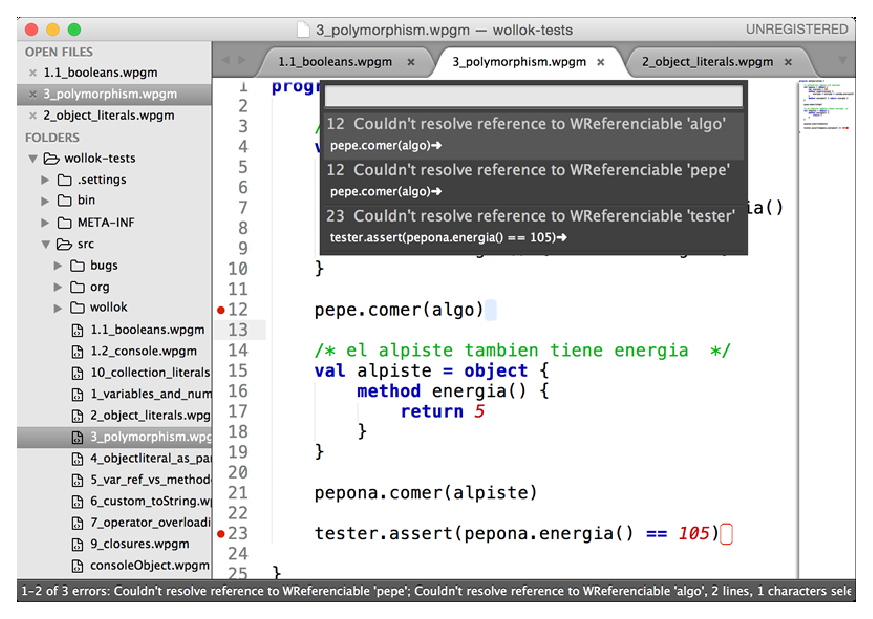
\includegraphics[height=0.8\textheight,natwidth=800,natheight=558]{images/wollok-wisit-sublime-linter.eps}
		\end{figure}
	\end{center}
}


%
% WOLLOK GAME
%

\section{Wollok Game}
\frame{
	\frametitle{Wollok Game}
	\begin{itemize}
		\item Herramienta complementaria al testeo unitario y consola interactiva.
		\item Mejorar la comprensión de conceptos.
		\item Visualización de comportamiento
		\item Motivación en el aprendizaje fomentando la participación.
	\end{itemize}
}

\frame{
	\frametitle{Wollok Game}
	\framesubtitle{FarmVille}
	\textbf{FarmVille} - Demo
	
	\begin{center}
		\begin{figure}
			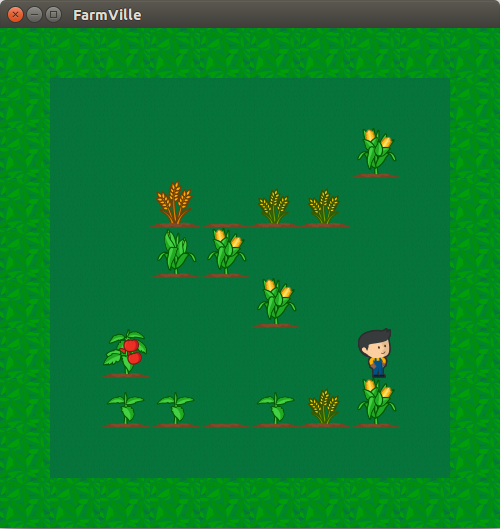
\includegraphics[width=0.4\textwidth,height=0.6\textheight,natwidth=500,natheight=529]{images/wollok-game-farmville.png}
		\end{figure}
	\end{center}
}

\frame{
	\frametitle{Wollok Game}
	\framesubtitle{Sokoban}
	\textbf{Sokoban} - Demo
	
	\begin{center}
		\begin{figure}
			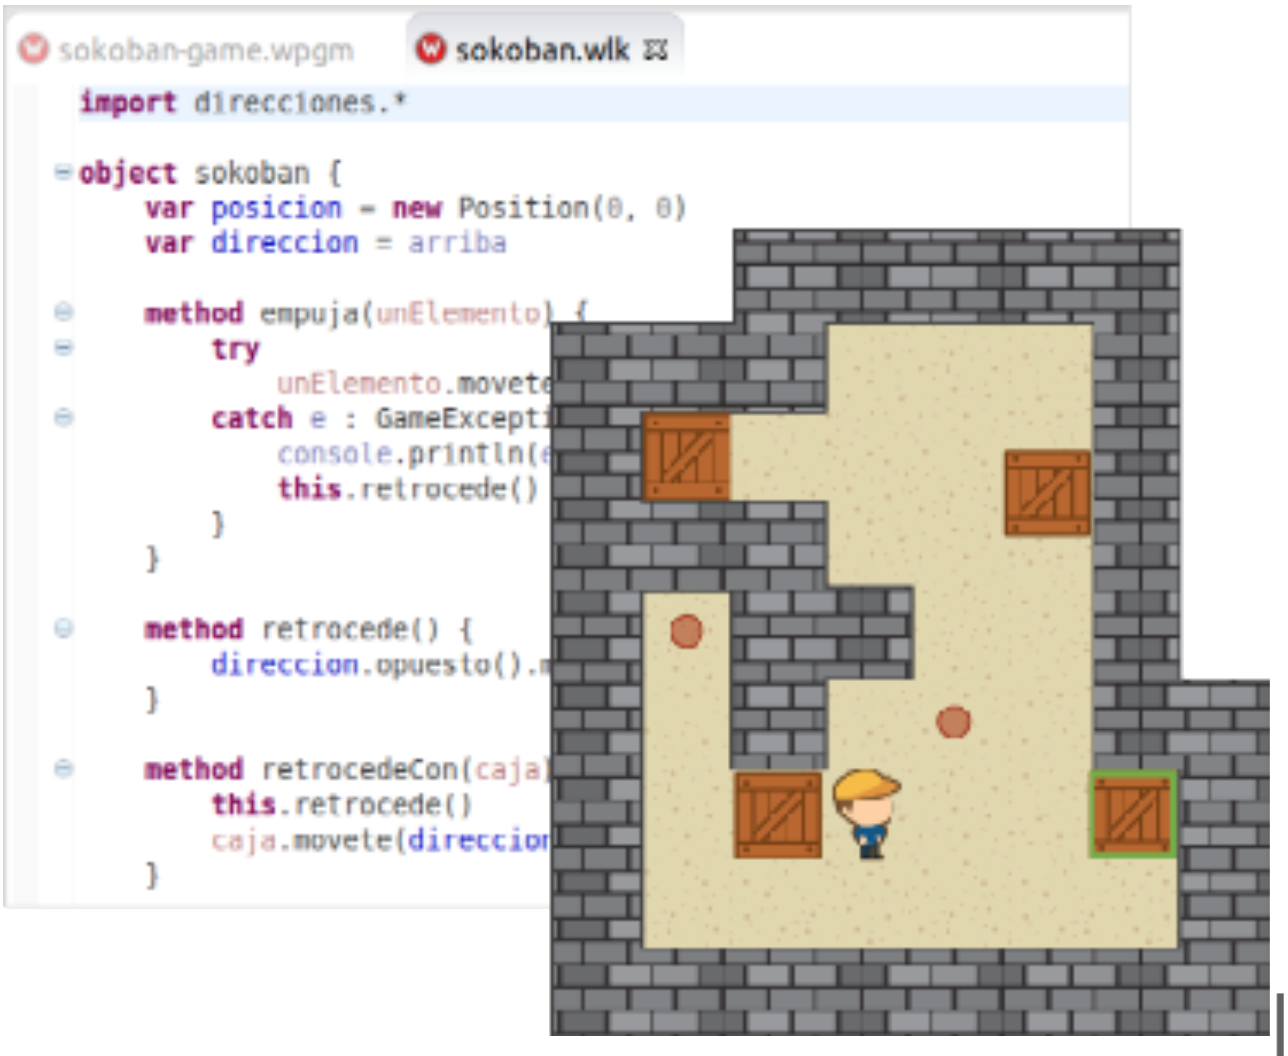
\includegraphics[width=0.4\textwidth,height=0.6\textheight,natwidth=258,natheight=289]{images/wollok-game-sokoban.png}
		\end{figure}
	\end{center}
}

\frame{
	\frametitle{Wollok Game}
	\framesubtitle{Futuro}
	Futuro
	\begin{itemize}
		\item + Tipos de \textbf{Juegos}
		\begin{itemize}
		  \item Survival
		  \item Por turnos
		\end{itemize}
		\item + Tipos de \textbf{Interacciones}
		\item Features Gráficos
		\begin{itemize}
		  \item Animaciones
		  \item Fondos infinitos
		  \item Distintos vistas (lateral, isométrica, etc)
		\end{itemize}
	\end{itemize}
}

\section{Experiencia en el Aula}
\frame{
	\frametitle{Experiencia en el Aula}
	Los alumnos se apropian intuitivamente de las herramientas
	\begin{itemize}
		\item Integración class-based / object-based
		\item El REPL resulta más intuitivo que los workspaces de Smalltalk
		\item Mayor control sobre los tests unitarios
		\item Editores
	\end{itemize}
	\pause
	\medskip
	\begin{center}
		Un \textbf{recorrido incremental} apoyado en \textbf{herramientas} adecuadas,\\
		\pause
		permite aprovechar la \textbf{intuición} del estudiante\\
		\pause
		fomentando su \textbf{autonomía, creatividad y motivación}\\
	\end{center}
}

\section{Próximos Pasos}
\frame{
	\frametitle{Próximos pasos}
	Próximos Pasos
	\begin{itemize}
		\item Varias discusiones sobre la mejor sintaxis
		\item Herencia basada en mixins
		\item Implementar wollok-game en el aula
		\item Plataforma p/interacción Alumno $ \leftrightarrow $ Docente 
	\end{itemize}
	
	Y muchas actividades para sumar más gente al proyecto.
}

\frame{
  \frametitle{Muchas gracias}.
  Muchas Gracias !
  \begin{center}
		\begin{figure}
			
\includegraphics[width=0.6\textwidth,height=0.6\textheight,natwidth=815,natheight=342]{images/logo-fun.png}
		\end{figure}
	\end{center}
}
\end{document}

